

\section{The example of lung cancer}
\label{Intro-lung}
\subsection{Lung cancer subtypes and etiology}
\begin{figure}[H]
    \centering
    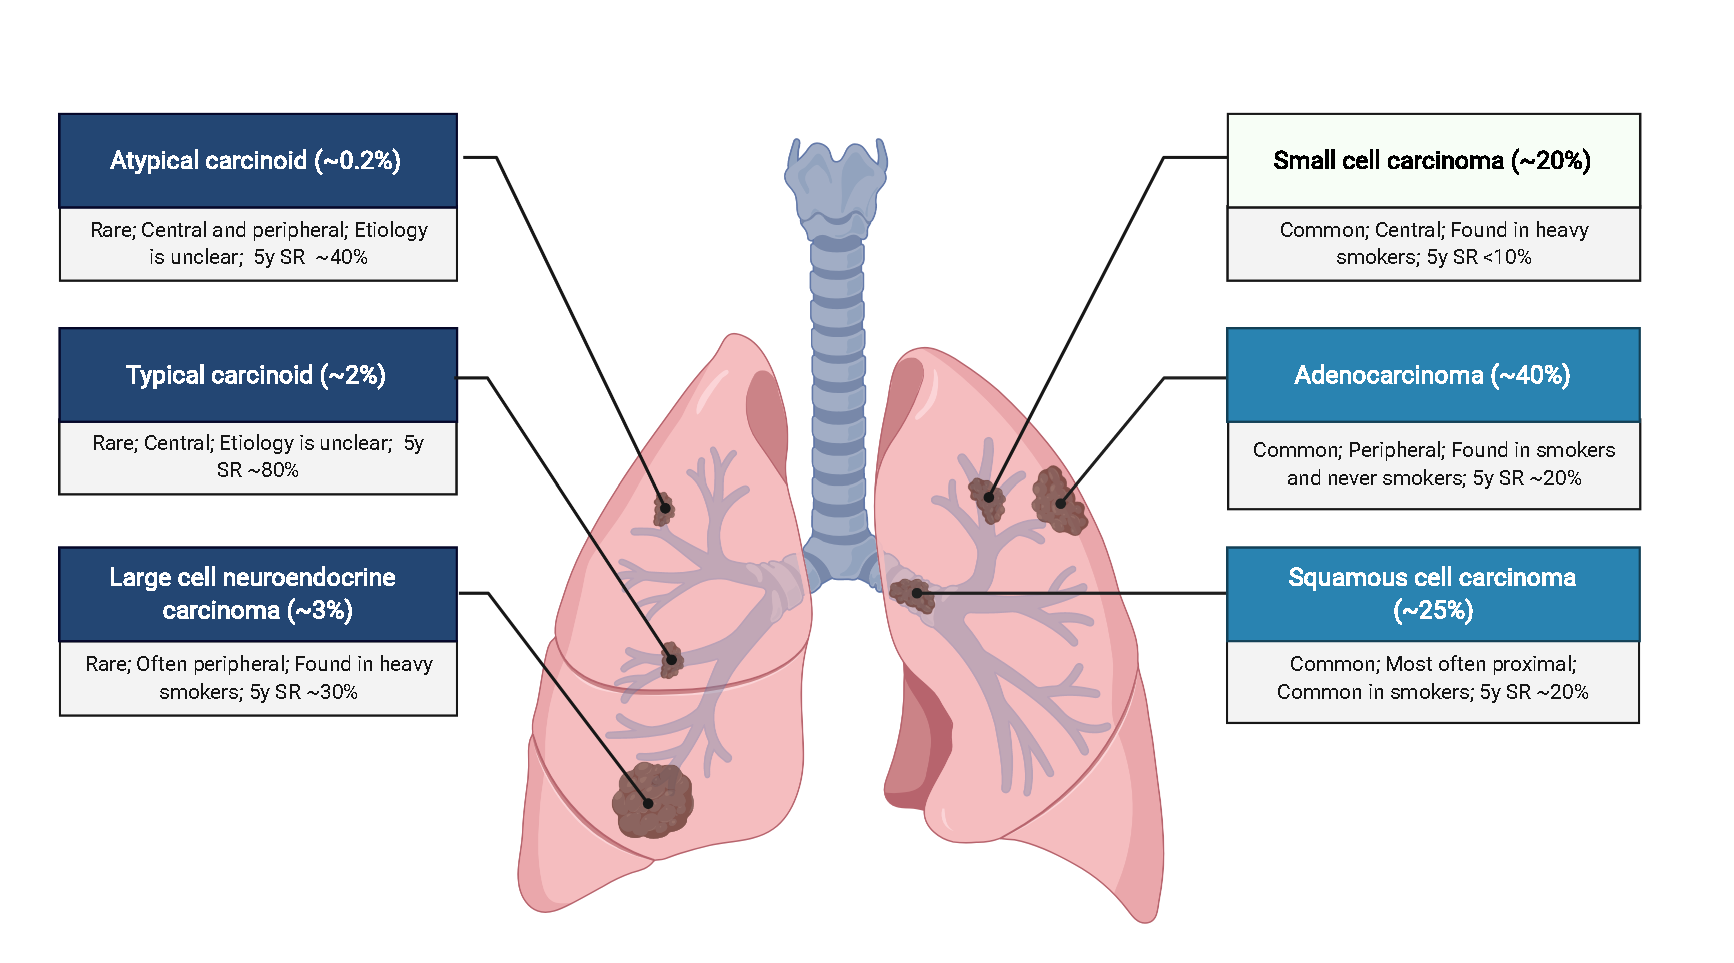
\includegraphics[width=1\textwidth]{Figures/Intro/Lung_cancer.pdf}
    \caption[Lung cancer subtypes]{\textbf{Lung cancer subtypes.} Each lung cancer type occurs at different frequencies as well as at distinct locations in the lung (from proximal to distal locations). Each box on the figure is associated to one cancer type and provides their characteristics (frequency, localisation, etiology and overall 5-year survival rate (5y SR)) \cite{Travis2010,Derks2018,Simbolo2019a,ASCO}. Figure created with \href{https://biorender.com/}{BioRender.com}}
    \label{fig:intro_lung}
\end{figure}
As mentioned at the beginning of the manuscript, lung cancer is one of the most common and deadliest cancer worldwide. Several subtypes of lung cancers have been identified (Figure \ref{fig:intro_lung}).
% Subtypes
The most common lung cancers are usually divided into two groups: the \gls{SCLC} and the \gls{NSCLC} samples, representing respectively around 20 and 75\% of the lung cancers \cite{Politi2015}. The second group is further separated into two main subgroups: the \gls{LUAD} and the \gls{LUSC}. Also, rarer forms of lung cancer exist. Multiple lung cancer subtypes, including such rarer cancers, were grouped in one category named the lung neuroendocrine tumors by the \gls{WHO} 2015 classification \cite{Travis2015}. This group comprises the pulmonary carcinoids, including the typical and atypical carcinoids, \gls{LCNEC} as well as the previously mentioned \gls{SCLC} tumors. 
Each lung cancer type can be distinguished by different etiologies, histopathological characteristics, molecular profiles and clinical outcomes (See Figure \ref{fig:intro_lung}).

%etiology
The strongest risk factor for lung cancer is smoking. Indeed, \gls{SCLC}s and \gls{LCNEC}s are frequently found in heavy smokers. Smoking is also a major risk factor for \gls{LUAD} and \gls{LUSC} cancers \cite{Campbell2016}. However, lung cancer can also develop in non-smokers. In particular, the \gls{LUAD} category corresponds to the lung cancer type most commonly found in never smokers. Although the etiology of the pulmonary carcinoids is not clear, the majority of these tumors are found in nonsmokers \cite{Derks2018}. %In addition, the smoking behaviour of patients from different subtypes can be different \cite{Pikor2013}...  
In addition, around only 15\% of smokers develop lung cancer suggesting than other factors mediate lung cancer risk. 

\subsection{Lung cancer susceptibility}
% Susceptibility
While exposures other than smoking like air pollution, radon, heavy metals or asbestos have been identified as lung cancer risk factors \cite{DeAlencar2020}, genetics is also contributing to the disease risk. In line with this hypothesis, it has been shown that having a family history of lung cancer confers a 2.5 fold lung cancer risk increase \cite{Amos1999}. Further evidence of lung cancer germline susceptibility has been revealed by \gls{GWAS} studies, with the identification of common variations associated with lung cancer. Genes involved in nicotine addiction (\textit{CHRNA} genes), telomere activities (\textit{TERT}) as well as genes related to the DNA repair and cell-cycle pathways (\textit{e.g.} \textit{Check2}, \textit{RAD52} or \textit{CDKN2A}) have been identified \cite{Bosse2018}. 
Also, some lung cancer associated variants were identified as related to the propensity to smoke \cite{Thorgeirsson2008,McKay2017} and genetic correlations between lung cancer and smoking traits, like smoking initiation, smoking cessation or smoking intensity have been described \cite{McKay2017}. Such observations provided evidence that susceptibility variants could influence lung cancer risk through environmental exposures.
Hence, \gls{GWAS} studies have enabled to gain insights on lung cancer etiology as well as on the biological pathways involved in the disease. However, the variants identified so far do not account for most of the heritability of lung cancer, estimated at 18\% and remaining today largely unexplained \cite{McKay2017}.  
%mention the ILCO consortium and TRICL
%inherited lung cancers \cite{DeAlencar2020}

\subsection{Lung cancer molecular profiling}
%mutational landscape
%Genetic studies like GWAS focus on germline genetics. 
In the past decades, molecular profiles of human tumors, including lung tumors, have also been explored thanks to the development of \gls{NGS} studies. Such studies have, for example, established that lung cancers are among the cancer types with the highest mutational burden (total number of mutations for a given part of \gls*{DNA}) \cite{Lawrence2013}.  
As mentioned in Section \ref{Intro-biology}, in smoking-related cancers, those mutations revealed a signature associated with tobacco consumption. Among the \gls{COSMIC} signatures identified by Alexandrov \textit{et al.} \cite{Alexandrov2013,Alexandrov2020}, the smoking signature corresponds to the Signature 4 (\gls{COSMIC} version 2) and SBS 4 (\gls{COSMIC} version 3). Those signatures are the results of \gls*{DNA} damages caused mainly by benzo[$\alpha$]pyrene, which is a mutagenic compound found in tobacco smoke and whose effects on \gls*{DNA} has been shown in experimental mutagenesis studies \cite{Nik-Zainal2015}. Even though smoking does heavily impact the lung tissue, it has been shown that quitting smoking can restore the damaged tissue \cite{Yoshida2020}.

In addition, molecular analyses of lung tumors have identified cancer driver genes in the different cancer types. Among those genes, the \textit{\gls{EGFR}} gene, which is part of the protein kinase family currently known to be mutated in around 15\% of the \gls{LUAD} samples \cite{Collisson2014}, has been related to therapeutic response in 2004 \cite{Politi2015}. Indeed LUAD samples, carrying activating mutations in the \textit{\gls{EGFR}} gene, are responsive to tyrosine kinase inhibitor therapy and have an improved survival in comparison to other cancer patients treated with chemotherapy. Such molecular studies largely influenced the way that lung tumors are classified since it is only since those discoveries that \gls{NSCLC} are further sub-classified. Guidelines were published in 2013 to include molecular testing, mainly based on \textit{\gls{EGFR}} and \textit{ALK} alterations testing, in the clinical practice for the \gls{NSCLC} patients. In 2018, those guidelines were updated and new alterations, like rearrangements in the tyrosine kinase \textit{ROS1}, are now recommended for molecular testing \cite{Lindeman2018}. In 2012 and 2014, the \gls{TCGA} marker papers on the two lung cancer cohorts (\gls{LUAD} and \gls{LUSC}) were published. The authors expanded the molecular profiling of these tumors and hence the list of drivers genes, improving the understanding of the biological mechanisms involved and providing new opportunities for patients management \cite{Network2012,Collisson2014}. Those studies also explored the transcriptomic, methylation and proteomic data from the lung tumors. Based on their expression profiles, the \gls{LUAD} tumors, were divided into subtypes that could help to refine those tumors classification \cite{Collisson2014}.

The identification of driver genes in lung cancer has also led to the proposal of molecular targets for early detection. The molecular profiling of \gls{SCLC}s is an example of such an application. \gls{SCLC}s are characterized by universal inactivation of both \textit{RB1} and \textit{TP53} genes \cite{Peifer2012a,George2015,Fernandez-Cuesta2019}. In 2016, Fernandez-Cuesta \textit{et al.} analyzed \gls{ctDNA}, which are fragments of tumor \gls*{DNA} released in the bloodstream that can be used as molecular biomarkers, in \gls{SCLC}s. They showed that \textit{TP53} mutations were detectable in the \gls{ctDNA} of the \gls{SCLC} cases \cite{Fernandez-cuesta2016}. 
\gls{ctDNA} applications are viable for multiple cancer types. In 2018, Cohen \textit{et al.} described a blood test called CancerSEEK, detecting proteins and mutations in cell-free \gls*{DNA} for the early detection of eight different cancer types, including lung cancer \cite{Cohen2018}. Such tests face though sensitivity issues due to the low abundance of mutated \gls*{DNA} in body fluids, hence adapted bioinformatics tools are needed. I contributed to the optimization of such tool, Needlestack, a highly sensitive multi-sample variant caller \cite{Delhomme2020}. 

Even though rare forms of lung cancers are less explored than the common lung cancers, recent molecular studies have started to characterize the lung neuroendocrine tumors as well \cite{Fernandez-Cuesta2014,George2018,Rekhtman2016,Simbolo2019}. Those studies have revealed that, on top of their histopathological differences, the lung neuroendocrine neoplasms were also distinct molecular entities \cite{Fernandez-Cuesta2019}. Low mutational burden has been observed in the atypical and typical pulmonary carcinoids in contrast to the highly mutated \gls{LCNEC}s and \gls{SCLC}s \cite{Derks2018}. Also, the transcriptomic profiling of those tumors has been investigated. These analyses identified molecular subgroups in different cancer types, revealing the molecular heterogeneity in those tumors \cite{George2018,Rudin2019}. The work described in chapters \ref{Chapter1} and \ref{Chapter2/4} of this thesis contributed to the molecular characterization of the lung neuroendocrine tumors.  \newline


The discoveries described in this section were enabled thanks to the large amount of data generated during the era of genomics (See Section \ref{Intro-ngs}). However, the analyses of these data have raised multiple challenges that required the use and development of specific computational methods. The next section intends to describe those aspects. 